\documentclass[sublist,a4paper,twoside,11pt]{article}
\usepackage[utf8]{inputenc}
\usepackage{a4wide}
%%% Various other
\usepackage{hyperref}
\hypersetup{
	colorlinks=true,
	linkcolor=blue,
	filecolor=magenta,      
	urlcolor=cyan,
}

\urlstyle{same}

\usepackage{amsmath}
\usepackage{breqn}
\usepackage{amssymb}
\usepackage{tabularx}
\usepackage{xltxtra}
%\usepackage{xgreek}
\usepackage{graphicx}

\usepackage{amsthm}

\author{André de Souza Mendes, N. Papadakis}
\title{Simple vehicle model 4dof }

\makeindex

% Definitions
\def\doubleunderline#1{\underline{\underline{#1}}}


\begin{document}
\maketitle
\tableofcontents
\section*{Nomeclature}

\begin{itemize}
\item [0]: Initial.
\item [A]: The Dynamic Matrix of the linear system.
\item [$\alpha$]: Distance from the point to [m].
\item [a]: Vector linear acceleration.
\item [B]: Matrix of linear system inputs.
\item [b]: Distance from the point[m].
\item [C]: Matrix of linear system outputs.
\item [D]: Linear system direct transmission matrix.
\item [E]: Observer sizing matrix (reference system)?
\item [e]: Observer error vector.
\item [C]: Damping $\left[\frac{N\cdot s}{rad}\right]$.
\item [ext]: External
\item [K]: lateral slope rigidity $\left[\frac{N\cdot m}{rad}\right]$.
\item [k]: Tire bend rigidity $\left[\frac{N}{rad}\right]$
\item [F]: force force module [N]
\item [F]: F force Vector
\item [f ]: Vector function.
\item [FD]: Refers to the point that locates the right front tire
\item [FE]: Refers to the point that locates the left front tire
\item [g]: Acceleration of gravity $[\frac{m}{s^2}]$
\item [h]: Height of the center of mass of the vehicle [m].
\item [I]: element of Inertial tersor $[kg^2]$.
\item [I]: Inertia Tensor.
\item [L]: Distance between tires on the same axle [m].
\item [M]: moment vector 
\item [M]: Mass [kg].
\item [n?]: Unit vector of the orthonormal base attached to the non-suspended element
\item [O]: The Point that locates the origin.
\item [P]: Weight force vector
\item [P]: Matrix transformation.
\item [P]: A point that locates a particular particle.
\item [r]: Vector position.
\item [RD]: Refererence to the point that locates the right rear tire.
\item [RE]: Refer to the point that locates the left rear tire.
\item [s]: Unit vector of the orthonormal base attached to the suspended mass.
\item [T]: Point that locates the center of mass of the vehicle.
\item [t]: Unit vector of the orthonormal basis fixed to the inertial frame
\item [U]: Input vector
\item [V]: Any matrix
\item [u]: Speed vector module $[\frac{m}{s}]$.
\item [v]: Linear velocity vector.
\item [w]: Vector of the unobservable part.
\item [w]: Angular velocity vector.
\item [x]: Refers to the longitudinal direction.
\item [x]: Vector of states.
\item [y]: Referring to the transverse direction.
\item [Y]: And Vector of outputs.
\item [z]: Referring to vertical direction
\item [b]: State vector of the observer (estimate)
\item [$\alpha$]: Drift angle [rad].
\item [$\delta$]: Steering angle [rad].
\item [$\Phi$]: Solidarity base the suspended mass
\item [$\phi$]: Tilt angle of vehicle [rad].
\item [$\Omega$]: Fixed base in the inertial frame.
\item [$\Psi$]: Solidarity base to the non-suspended element.
\item [$\psi$]: Vehicle orientation angle [rad].
\end{itemize}


\section{MODEL}
\subsection{Tire Model}
The tire model used relates linearly the lateral force of the tire to its drift angle. That is
\begin{equation}
F=-k*\alpha
\end{equation} 

\subsection{Vehicle Model}
The physical vehicle model used is shown in \ref{fig:vehiclemodel}. The system has four degrees of freedom: 
\begin{itemize}
\item two coordinates positioning the point P, 
\item the orientation of the vehicle in the horizontal plane $\psi$ 
\item and the slope angle $\phi$.
\end{itemize}
	
	\begin{figure}
		\centering
		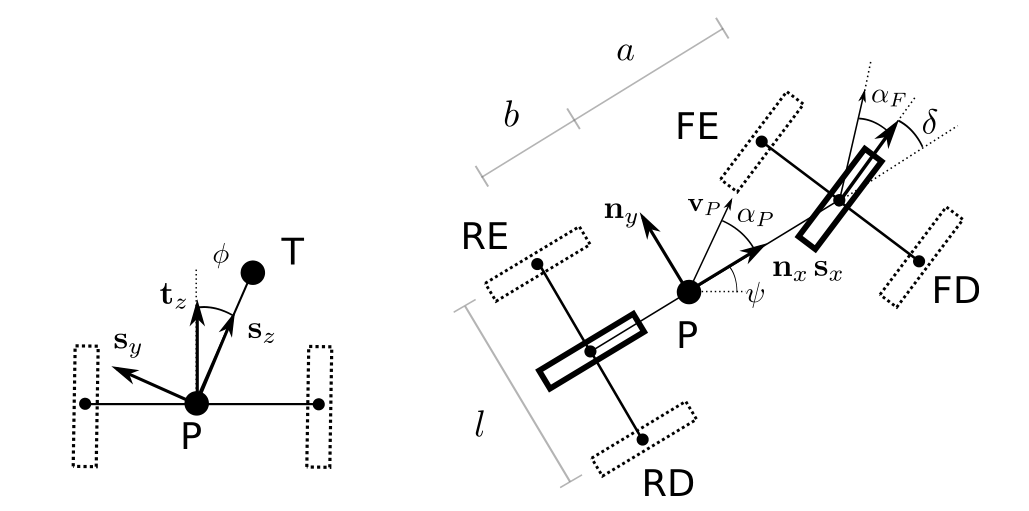
\includegraphics[width=0.7\linewidth]{figures/VehicleModel}
		\caption{Vehicle Model }
		\label{fig:vehiclemodel}
	\end{figure}
	

	
	
The bases used are $\Omega = \{O,t_x, t_y, t_z \}$, $\Psi = \{P, n_x, n_y, n_z \}$ and $\Phi = \{P,s_x s_y,s_z\}$. A base $\{O,t_x, t_y,t_z \}$ is fixed to the inertial frame. The origin is given by the point 0 and the vectors $t_x, t_y$ and $t_z$ point to the longitudinal, transverse and vertical directions, respectively. Reference system $\{P, n_x, n_y, n_z\}$ is coupled to the non-suspended element. The origin coincides with point P which exists in the plane defined by vectors $t_x$ and $t_y$. The vector $n_x$ forms an angle $\psi$ with the vector $t_x$ and the vector $t_z$ is parallel to the vector $n_z$. The base = $\{P,s_x, s_y,s_z\}$. also has origin coincident with point P. The vector $n_x$ is parallel to the vector $s_x$. The vector $s_z$ forms an angle $\phi$ with respect to the vector $n_z$. The angular coordinate $\alpha_P$ indicates the orientation of the velocity vector $v_P$ with respect to the axis longitudinal direction of the non-suspended element.
	
\subsubsection{Non-linearity}

The velocity vector of the point P is given by

\begin{equation}
	\label{eq:2.P.velocity.vector}
V_P = v_p\cdot \cos(\alpha_P) n_x + v_p\cdot \sin(\alpha_P ) n_y
\end{equation}

And the position vectors of the points that locate the four tires of the vehicle (FD, FE, RD and RE) with respect to point P are given by

\begin{subequations}
	\label{eq:3.wheel.radius.vector}
	\begin{equation}
	r_{FD/P} = \alpha n_x - \frac{l}{2}n_y
	\end{equation}
	\begin{equation}
		r_{FE/P} = \alpha n_x  + \frac{l}{2}n_y
	\end{equation}
	\begin{equation}
		r_{RD/P} = -b n_x - \frac{l}{2}n_y
	\end{equation}
	\begin{equation}
		r_{RE/P} = -b n_x + \frac{l}{2}n_y
	\end{equation}
\end{subequations}


The velocity vectors on each wheel can be written as

\begin{subequations}
	\label{eq:4.wheel.velocity.vector}
\begin{equation}
\mathbf{v}_{FD}=v_P+w_\Psi \times r_{FD/P}	
\end{equation}
\begin{equation}
\mathbf{v}_{FE}=v_P+w_\Psi \times r_{FE/P}	
\end{equation}
\begin{equation}
\mathbf{v}_{RD}=v_P+w_\Psi \times r_{RD/P}	
\end{equation}
\begin{equation}
\mathbf{v}_{RE}=v_P+w_\Psi \times r_{RE/P}	
\end{equation}

\end{subequations}


Substituting the equations in (\ref{eq:3.wheel.radius.vector}) into (\ref{eq:4.wheel.velocity.vector}), results in ($\omega_{\Psi}=\dot{\psi}$): 

\begin{subequations}
	\begin{equation}
	\mathbf{v}_{FD}=\left(v_P \cos(\alpha_P) +\frac{l}{2}\dot{\psi}\right)n_x +\left(v_P \sin(\alpha_P) +\alpha \dot{\psi}\right)n_y
	\end{equation}
	\begin{equation}
	\mathbf{v}_{FE}=\left(v_P \cos(\alpha_P) -\frac{l}{2}\dot{\psi}\right)n_x +\left(v_P \sin(\alpha_P) +\alpha \dot{\psi}\right)n_y
	\end{equation}
	\begin{equation}
	\mathbf{v}_{RD}=\left(v_P \cos(\alpha_P) +\frac{l}{2}\dot{\psi}\right)n_x +\left(v_P \sin(\alpha_P) -b \dot{\psi}\right)n_y
	\end{equation}
	\begin{equation}
	\mathbf{v}_{RE}=\left(v_P \cos(\alpha_P) -\frac{l}{2}\dot{\psi}\right)n_x +\left(v_P \sin(\alpha_P) -b \dot{\psi}\right)n_y
\end{equation}
\end{subequations}


Therefore, the drift angles in each tire are given by	
\begin{subequations}
\begin{equation}
	a_{FD}=\arctan\left(\frac{v_P \sin(\alpha_P) +\alpha \dot{\psi}}{v_P \cos(\alpha_P) +\frac{l}{2}\dot{\psi}}  \right)-\delta
\end{equation}
\begin{equation}
	a_{FE}=\arctan\left(\frac{v_P \sin(\alpha_P) +\alpha \dot{\psi}}{v_P \cos(\alpha_P) -\frac{l}{2}\dot{\psi}}  \right)-\delta 
	\end{equation}
	\begin{equation}
	a_{RD}=\arctan\left(\frac{v_P \sin(\alpha_P) -b\dot{\psi}}{v_P \cos(\alpha_P) +\frac{l}{2}\dot{\psi}}  \right)
	\end{equation}
	\begin{equation}
	a_{RE}=\arctan\left(\frac{v_P \sin(\alpha_P)  -b\dot{\psi}}{v_P \cos(\alpha_P) -\frac{l}{2}\dot{\psi}}  \right) 
	\end{equation}
\end{subequations}

The velocity vector of the center of mass is given by

\begin{equation}
v_T = v_P + \omega_\Phi\times r_{T/P}
\end{equation}

where $r_{T/P} = h \vec{s}_z =  - h(\sin(\phi) \vec{n}_y + \cos(\phi) \vec{n}_z )$

Where the orientation change of the base $\Phi$ is given by

\begin{equation}
\omega_\Phi = \dot{\phi} n_x + 0 n_y+ \dot{\psi} n_z
\end{equation}

The change of orientation of the base $\Phi$ is given by	

\begin{equation}
\omega_\Psi = \dot{\psi} n_z
\end{equation}

Then the velocity vector of point T is

\begin{equation}\label{eq:10.velocity.vector}
v_T = (v_P \cdot \cos(\alpha_P) +\dot{\psi} h \sin(\phi)   )nx +
(v_P \cdot \sin(\alpha_P) - \dot{\phi} h \cos(\phi))ny
+(-\dot{\phi} h  sin(\phi))nz
\end{equation}

By differentiating equation (\ref{eq:10.velocity.vector}) we obtain 

\begin{dmath}
	\label{eq:11.T.acceleration.vector}
a_T = (\dot{v}_P \cos(\alpha_P) - v_P(\dot{\psi}+\dot{\alpha}_P)\sin(\alpha_p)+ \ddot{\psi} h \sin(\phi) + 2h\dot{\psi}\dot{\phi})nx +
%
(\dot{v}_P \sin(\alpha_P) + v_P(\dot{\psi}+\dot{\alpha}_P)\sin(\alpha_p) -  \ddot{\phi} h \cos(\phi) +  h (\dot{\psi}^2+\dot{\phi}^2)\sin(\phi))ny
%
+(-h\ddot{\phi}\sin(\phi) - h\dot{\phi}^2\cos(\phi) )nz
\end{dmath}


The forces on the four tires are given by:

\begin{subequations}
	\begin{equation}
	F_{FD} = (F_{FD,x}\cdot \cos(\delta) - F_{FD,y}\cdot \sin(\delta) ) n_x + (F_{FD,x}\cdot \sin(\delta) - F_{FD,y}\cdot \cos(\delta) ) n_y 
	\end{equation}
	\begin{equation}
	F_{FE} = (F_{FE,x}\cdot \cos(\delta) - F_{FE,y}\cdot \sin(\delta) ) n_x + (F_{FE,x}\cdot \sin(\delta) - F_{FE,y}\cdot \cos(\delta) ) n_y
	\end{equation}
	\begin{equation}
	F_{RD} = F_{RD,x} n_x + F_{RD,y} n_y
	\end{equation}
	\begin{equation}
	F_{RE} = F_{RE,x} n_x + F_{RE,y} n_y
	\end{equation}
	\label{eq:12_tire_forces}
\end{subequations}

At this point it is important to note that the vertical force in each tire is the bonding force that maintains the contact point of the tires contained in the horizontal plane.

The theorem of the barycentre movement is given by

\begin{equation}
m\cdot \vec{a} = \sum F_{ext} \label{eq:13_barycenter}
\end{equation}

Substituting equations (\ref{eq:11.T.acceleration.vector}) and (\ref{eq:12_tire_forces}) into (\ref{eq:13_barycenter}), in the $n_x$ direction we have	

\begin{dmath}	\label{eq:14.nx.translational.motion}
	m\left( \dot{v}_P \cos (\alpha_P) - v_P(\dot{\psi}+\dot{\alpha}_P) \sin (\alpha_P) + \ddot{\psi} h \sin{\phi} + 2 h \dot{\psi}\dot{\phi}\cos(\phi)\right)= 
      (F_{FD,x}+F_{FE,x})\cos(\delta) - (F_{FD,y}+F_{FE,y})\sin(\delta) + (F_{RD,x}+F_{RE,x})
\end{dmath}

And in the direction $n_y$ we have

\begin{dmath}\label{eq:15.ny.translational.motion}
	m\left( \dot{v}_P \sin(\alpha_P) - v_P(\dot{\psi}+\dot{\alpha}_P) \sin (\alpha_P) - \ddot{\phi} h \cos{\phi} + 2 h (\dot{\psi}^2+\dot{\phi}^2) \sin(\phi)\right)= 
	(F_{FD,x}+F_{FE,x})\sin(\delta) + (F_{FD,y}+F_{FE,y})\cos(\delta) + (F_{RD,x}+F_{RE,x})
\end{dmath}
	

The position of the point T in relation to the point P in the base $\Phi$ is:

\begin{equation}
\label{eq:16.T.position.vector}
\vec{r}_{T/P}  = h \vec{s}_z
\end{equation}


In addition, the acceleration of the point P is obtained by deriving with respect to time equation (\ref{eq:2.P.velocity.vector}). Writing the result on the basis $\Phi$ we have

\begin{dmath}	\label{eq:17.P.acceleration.vector.wrt.Pbase}
a_P = \left(\dot{v}_P \cos(\alpha_P) - v_P(\dot{\psi}+\dot{\alpha}_P)\sin(\alpha_p)\right)\vec{s}_x+ 
%
\left(\dot{v}_P \sin(\alpha_P)\cos(\phi) + (\dot{\psi}+\dot{\alpha}_P)\cos(\alpha_P)\cos(phi) \right) \vec{s}_y
%
- \left(\dot{v}_P \sin(\alpha_P)\cos(\phi) + v(\dot{\psi}+\dot{\alpha}_P)\cos(\alpha_P)\sin(phi) \right) \vec{s}_z
\end{dmath}

The vector $\omega_\Phi$ written on the basis $\Phi$ is given by	

\begin{equation}	\label{eq:18.omega_phi.wrt.Pbase}
\omega_\Phi = \dot{\phi}\vec{s}_x + \dot{\psi}\sin(\phi)\vec{s}_y + \dot{\psi}\cos(\phi)\vec{s}_z
\end{equation}

By differentiating equation (\ref{eq:18.omega_phi.wrt.Pbase}) with respect to time we have

\begin{equation}
\label{eq:19.dot_omega_phi.vector}
\dot{\omega}_\Phi = \ddot{\phi}\vec{s}_x + (\dot{\psi}\dot(\phi)\cos(\phi) + \ddot{\psi}\sin(\phi)) \vec{s}_y + 
(-\dot{\psi}\dot{\phi}\sin(\phi) + \ddot{\psi}\cos(\phi))\vec{s}_z
\end{equation}

The moments of the external forces with respect to point P are given by:

\begin{subequations}
		\label{eq:20.wheel.moments.due.to.externalforces}
	\begin{equation}
	M_{FD} = r_{FD/P} \times F_{FD}
	\end{equation}
	\begin{equation}
	M_{FE} = r_{FE/P} \times F_{FE}
	\end{equation}
	\begin{equation}
	M_{RD} = r_{RD/P} \times F_{RD}
	\end{equation}
	\begin{equation}
	M_{RE} = r_{RE/P} \times F_{RE}
	\end{equation}
\end{subequations}


Substituting equations (\ref{eq:3.wheel.radius.vector}) and (\ref{eq:12_tire_forces}) into (\ref{eq:20.wheel.moments.due.to.externalforces}) and writing the result into the base


\begin{subequations}\label{eq:21.wheel.moments}
	\begin{dmath}
	M_{FD} =   \sin(\phi) \left( a F_{FD,x} \sin(\delta) + a F_{FD,y} \cos(\delta) +  \frac{l}{2} F_{FD,x} \cos(\delta)  - \frac{l}{2} F_{FD,y} \sin(\delta) \right) \vec{s}_y + 
	%
	\cos(\phi) \left( a F_{FD,x} \sin(\delta) + a F_{FD,y} \cos(\delta) +  \frac{l}{2} F_{FD,x} \cos(\delta)  - \frac{l}{2} F_{FD,y} \sin(\delta) \right) \vec{s}_z  
	\end{dmath}
	\begin{dmath}
	M_{FE} =   \sin(\phi) \left( a F_{FE,x} \sin(\delta) + a F_{FE,y} \cos(\delta) -  \frac{l}{2} F_{FE,x} \cos(\delta)  + \frac{l}{2} F_{FE,y} \sin(\delta) \right) \vec{s}_y + 
	%
	\cos(\phi) \left( a F_{FE,x} \sin(\delta) + a F_{FE,y} \cos(\delta) - \frac{l}{2} F_{FE,x} \cos(\delta)  + \frac{l}{2} F_{FE,y} \sin(\delta) \right) \vec{s}_z 	\end{dmath}
	\begin{dmath}
	M_{RD} =   \sin(\phi)\left(- b F_{RD,y} +  \frac{l}{2} F_{RD,x} + \right)\vec{s}_y + \cos(\phi)\left(- b F_{RD,y} +  \frac{l}{2} F_{RD,x} + \right)\vec{s}_z 
	\end{dmath}
	\begin{dmath}
	\sin(\phi)\left(- b F_{RE,y} -  \frac{l}{2} F_{RD,x} + \right)\vec{s}_y + \cos(\phi)\left(- b F_{RE,y} -  \frac{l}{2} F_{RE,x} + \right)\vec{s}_z 
	\end{dmath}
\end{subequations}


The moment generated by the force weight is given by

\begin{equation}\label{eq:22.weight.moment.vector}
M_P = r_{T/P}\times P = (-h   \sin(\phi) n_y + h \cos(\phi) n_z )\times (-mg) n_z  = m g h  \sin(\phi) n_x = m g h  \sin(\phi) s_x 
\end{equation}

And the moment generated by the torsional spring is

\begin{equation}\label{eq:23.torsionalspring.moment.vector}
M_k = - K \phi s_x
\end{equation}

Finally, the moment generated by the damping is

\begin{equation}\label{eq:24.damping.moment.vector}
M_k = - C \dot{\phi} s_x
\end{equation}

The inertia tensor with respect to point P and written on the basis $\Phi$ is given by

\begin{equation}\label{eq:25.InertiaTensor.wrt.P}
I_p = \begin{bmatrix}
 I_{xx} & -I_{xy} & -I_{xz} \\
-I_{yx} &  I_{yy} & -I_{yz} \\
-I_{zx} & -I_{zy} &  I_{zz} 
\end{bmatrix}
\end{equation}


The angular motion theorem in relation to the point P is given, in matrix form, by
\begin{equation}\label{eq:26.wheel.velocity.vector}
m\;\doubleunderline{r_{T/P}} \;\underline{a_{P}} +  \doubleunderline{\omega_{\Phi}} \; \underline{I_{P}}\; \underline{\Phi} + \underline{I_P} \; \underline{\dot{\omega}_{\Phi}} = \sum \underline{M_{ext,P}} 
\end{equation}

Where the simple underline notation indicates a double column and underline matrix indicates a square matrix. The square matrices representing vectors follow the following construction

\begin{equation}
\doubleunderline{\xi_x q_x + \xi_y q_y + \xi_z q_z} = 
\begin{bmatrix}
0  & -\xi_{z} & \xi_{y} \\
\xi_{z}  &      0  & -\xi_{x} \\
-\xi_{y}  & \xi_{x} &  0 
\end{bmatrix}
\end{equation}

Where $q$ are the unit vectors of any base.
Then, by substituting equations \ref{eq:16.T.position.vector}, \ref{eq:17.P.acceleration.vector.wrt.Pbase}, \ref{eq:18.omega_phi.wrt.Pbase}, \ref{eq:19.dot_omega_phi.vector}, \ref{eq:21.wheel.moments}, \ref{eq:22.weight.moment.vector}, \ref{eq:23.torsionalspring.moment.vector}, \ref{eq:24.damping.moment.vector} and \ref{eq:25.InertiaTensor.wrt.P} in (\ref{eq:26.wheel.velocity.vector}) we obtain in the direction sx

\begin{dmath}\label{eq:28.sx.angular.motion.equation}
 I_{xx} \ddot{\phi} - I_{xz} \dot{\psi}^2\cos(\phi)  - I_{xz} \ddot{\phi}\cos(\phi)  - I_{xy} \ddot{\phi}\sin(\phi)
 +\frac{(I_{zz}-I_{yy}) \dot{\psi}^2 \sin(2\phi)}{2} + 2 I_{yz} \dot{\psi}^2\cos^2(\phi)-  \dot{v}_p h m 
  \cos(\phi)\sin(a_P) - \left(\dot{a}_P + \dot{psi}\right) h m v_p \cos(a_P)\cos(\phi)    =  m g h  \sin(\phi) s_x - K\phi - C \dot{\phi}
\end{dmath}

And in the direction sz

\begin{dmath}\label{eq:29.sz.angular.motion.equation}
	I_{zz} ( \ddot{\phi} \cos (\phi) -\dot{\phi}\dot{\psi} \sin(\phi) ) 
	- \dot{\phi} ( I_{xy}  \dot{\phi}+  I_{xx} \dot{\psi}\sin(\phi) )  \\
	+ \dot{\psi}  \sin(\phi)( I_{yy}\dot{\phi} +  I_{xy} \dot{\psi}  \sin(\phi)) 
	- \dot{\psi}  \cos(\phi)( I_{yz}\dot{\phi} +  I_{xz} \dot{\psi}  \sin(\phi)) \\
	- I_{yz} ( \ddot{\psi} \sin(\phi) -\dot{\phi}\dot{\psi} \sin(\phi) )
	- I_{zz}\ddot{\phi}   \\
	= \cos(\phi) a ( F_{FD,x} +  F_{FE,x})  \sin(\delta)
	+ a ( F_{FD,y} +  F_{FE,y})  \cos(\delta)
	+ \frac{l}{2}( F_{FD,x} -  F_{FE,x})  \cos(\delta)
	+ \frac{l}{2}( -F_{FD,y} +  F_{FE,y})  \sin(\delta)  \\
	+ \cos(\phi)  
	- b ( F_{RD,y} + F_{RE,y})
	- b ( F_{RD,y} + F_{RE,y})
\end{dmath}


Therefore, the equations of motion of the system are given by equations (\ref{eq:14.nx.translational.motion}), (\ref{eq:15.ny.translational.motion}), (\ref{eq:28.sx.angular.motion.equation}) and (\ref{eq:29.sz.angular.motion.equation})

\subsection{Linearisation}
This model presents the variables and time derivatives $\dot{\psi} ,\ddot{\psi} u,\dot{u}, \phi,\dot{\phi},\ddot{\phi},a_P$  and $\dot{a}_p$.  Therefore, the dynamic equations (\ref{eq:14.nx.translational.motion}), (\ref{eq:15.ny.translational.motion}), (\ref{eq:28.sx.angular.motion.equation}) and (\ref{eq:29.sz.angular.motion.equation}) can be used to write explicitly the Temporal derivatives $\ddot{\psi}, \dot{u}, \dot{a}_p$ and $\dot{\phi}$ as a function of the other variables and derivatives. So the model becomes:

\begin{equation}\label{eq:30.model}
\begin{bmatrix} 
	\dot{a}_P   \\ 
	\dot{v}       \\ 
	\ddot{\phi} \\ 
	\ddot{\psi} 
\end{bmatrix}
=f( \dot{\psi},v,\phi,\dot{\phi}, a_P )     
\end{equation}


Then the model is linearized at a given point of operation. In this report, all the inputs, $F_{FD,x}, F_{FE,x}, F_{RD,x}, F_{RE,x}$, and $\delta$ are considered zero. Then, linearization is performed by truncating the Taylor series expansion of equation (\ref{eq:30.model}). In this form, the velocity vector module $u_P$ remains constant, so in the differential equation the corresponding to $\dot{u}_P$ is discarded.
The linearized model can be written in state space. In matrix form


\begin{eqnarray}\label{eq:31.linearised.model.state.space}
\dot{x} = Ax + Bu \nonumber\\
y = Cx + Du
\end{eqnarray}

Where states are given by:

\begin{equation}\mathbf{x}=
\begin{bmatrix}
a_P\\
\dot{phi}\\
\dot{psi}\\
\phi
\end{bmatrix}
\end{equation}

The output vector consists of the two angular accelerations, $\ddot{\psi}$ and $\ddot{\phi}$, which are the two measured quantities of the system. That is, the matrix C is composed of lines 2 and 3 of matrix A, so it has a 2 × 4 dimension.
The data used in the numerical integration are presented in table 1. The eigenvalues of the system, in this case are given by

\begin{verbatim}
-9.6448 + 6.1884i
-9.6448 - 6.1884i
-9.3713 + 0.0000i
-2.3273 + 0.0000i
\end{verbatim}

Moreover, in this situation, the (A, C) is completely observable, since the observability matrix is 

\begin{equation}Obs=
\begin{bmatrix}
\mathbf{C}\\
\mathbf{CA}\\
\mathbf{CA^2}\\
\mathbf{CA^3}
\end{bmatrix}
\end{equation}


presents full position.


\begin{table}[h]	
	\centering
	\caption{Vehicle Parameters}	\label{table:Vehicle.Parameters}
	\begin{tabular}{|c|l|c|c|}
		\hline
Item & Description & Value & Unit \\
\hline
$m$ & Vehicle mass & 1000 & kg\\
$a$ & Distance between the point P and the front axle & 1.2 & m\\
$b$ & Distance between the point P and the rear axle & 1 & m\\
$h$ & 2eight of center of mass & 0.5 & m\\
$l$ & Distance between tires on the same axle & 0.8 & m\\
$K$ & Rigidity of lateral tilt & 100,000 & $\frac{N\cdot  m}{ rad}$\\
$C$ & Sidewall damping & 10,000 & $\frac{N \cdot m}{ rad}$\\
$k$ & Coefficient of curve stiffness & 10,000 & $\frac{N}{ rad}$\\
$I_{xx}$ & Moment of inertia & 800 & $kg\cdot m^2$\\
$I_{yy}$ & Moment of inertia & 1000 & $kg\cdot m^2$\\
$I_{zz}$ & Moment of inertia & 1000 & $kg\cdot m^2$\\
$I_{xy}$ & Product of inertia & 200 & $kg\cdot m^2$\\
$I_{xz}$ & Product of inertia & 200 & $kg\cdot m^2$\\
$I_{yz}$ & Product of inertia & 200 & $kg\cdot m^2$\\
$V_P$ & P-point speed & 10 & m / s\\
\hline
	\end{tabular}
\end{table}


The evolution of the states to an initial condition given by

\begin{equation}\mathbf{x}=
\begin{bmatrix}
a_{P,0}\\
\dot{\phi}_{0}\\
\dot{\psi}_{0}\\
\phi_{0}
\end{bmatrix}  = 
\begin{bmatrix}
0.5\\
-0.2\\
0.3\\
0.1
\end{bmatrix}
\end{equation}

is shown in figure \ref{fig:stateevolution}. In this figure it is possible to observe that all states converge to zero at a simulation time of less than two seconds.


\begin{figure}[h]
	\centering
	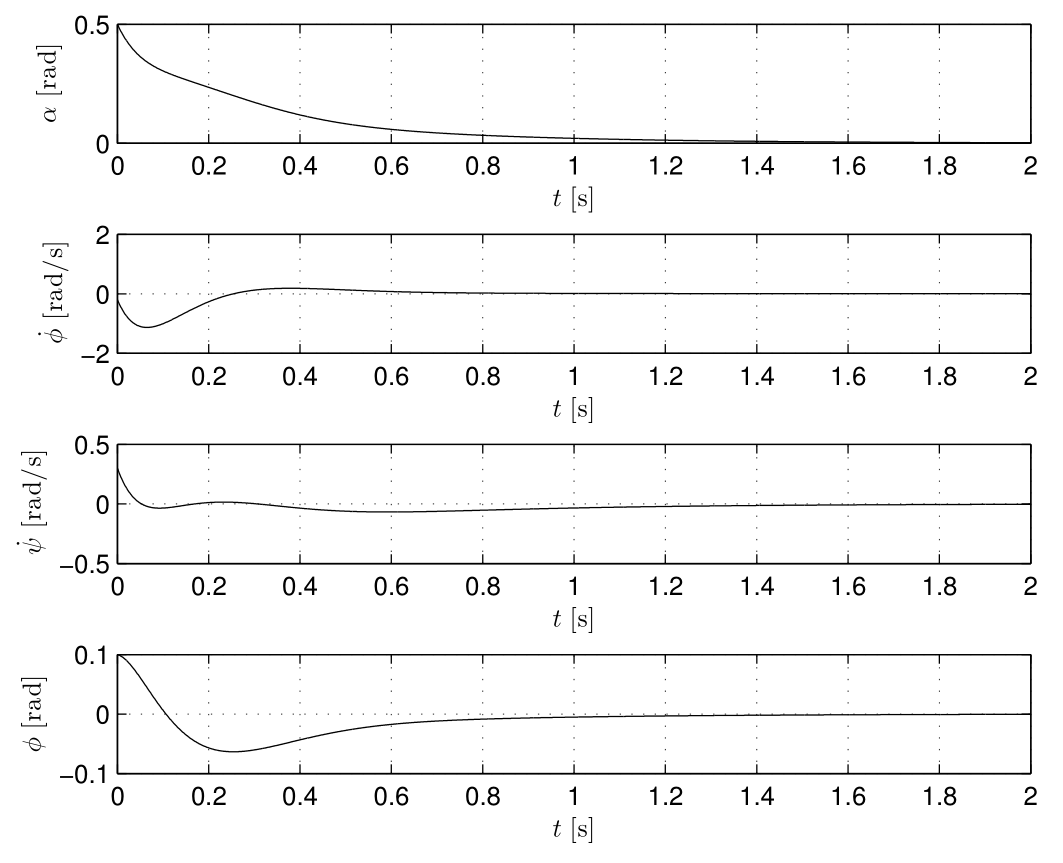
\includegraphics[width=0.9\linewidth]{figures/StateEvolution}
	\caption{Evolution of the states for a given initial condition}
	\label{fig:stateevolution}
\end{figure}


\section{OBSERVER IDENTITY}
The configuration of the states of a given dynamic system can be obtained from the measurement of the system variables through sensors. However, in many practical situations, direct measurement of states is not possible because of its inaccessible condition. To circumvent this limitation we apply the so-called state observers. These mathematical models estimate the configuration of the states from the measurements that were made. In Figure \ref{fig:observeridentityblockdiagram} it is possible to observe the block diagram of the identity state observer. This observer estimates, from the measurements, the dynamic condition of the states that compose the system 

\begin{figure}
	\centering
	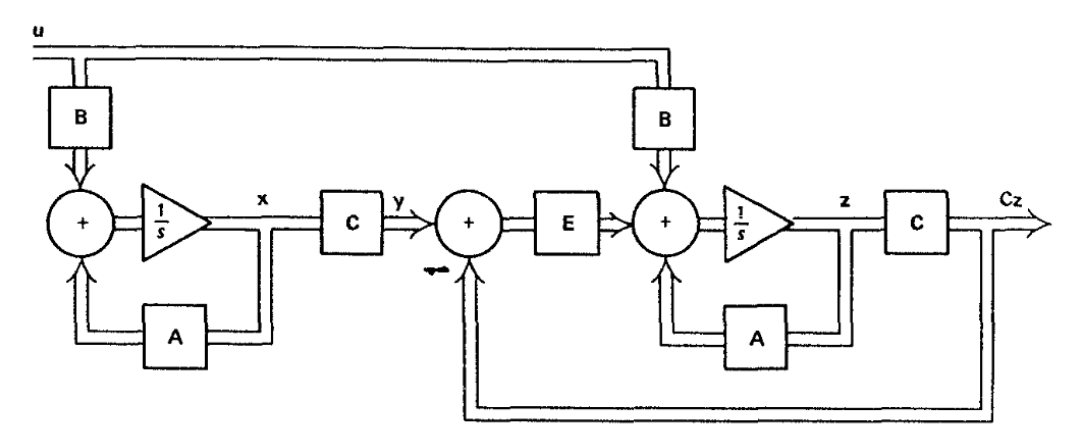
\includegraphics[width=0.7\linewidth]{figures/ObserverIdentityBlockDiagram}
	\caption{Block diagram of the plant with the observer identity}
	\label{fig:observeridentityblockdiagram}
\end{figure}


It is possible to observe that the dynamic equation of the observer is given by

\begin{equation}\label{eq:35.observer.dynamic.equation}
\mathbf{\dot{z} = (A-EC)z+ Ey+Bu}
\end{equation}

where $\mathbf{y}$ is the vector of measured variables of the plant and $\mathbf{u}$ is the input vector. In this case, both are considered inputs from the observer model.
Comparing equations (\ref{eq:31.linearised.model.state.space}) and (\ref{eq:35.observer.dynamic.equation}) it is possible to show that

\begin{equation}\label{eq:36.error.rate}
\mathbf{\dot{e} = (A-EC)e}
\end{equation}


That is, $\mathbf{e = z-x}$ is equal to the estimation error. Through the matrix $\mathbf{E}$, arbitrary, the eigenvalues of $\mathbf{(A - EC)}$ are adjusted. When the poles of equation (\ref{eq:36.error.rate}) lie to the left of the imaginary axis the error converges to zero. The poles of the identity observer were chosen:

\begin{verbatim}
-96.4481 +61.8839i
-96.4481 -61.8839i
-93.7131 + 0.0000i
-23.2730 + 0.0000i
\end{verbatim}

Matrix $\mathbf{E}$ is obtained by the \emph{place} command of the Matlab program.

The performance of the identity observer can be observed in figure \ref{fig:observeridentityperformance}. In this figure, the full lines represent the evolution of the states for the same integration shown in figure \ref{fig:stateevolution} and the dashed lines indicate the estimates of the states z obtained integrating the equation (\ref{eq:35.observer.dynamic.equation}) with input u null and y with the plant measurement information. It is possible to observe that in less than 0.2 seconds the estimated states assume the same values of the integration states of the linear model that simulates the system.


\begin{figure}
	\centering
	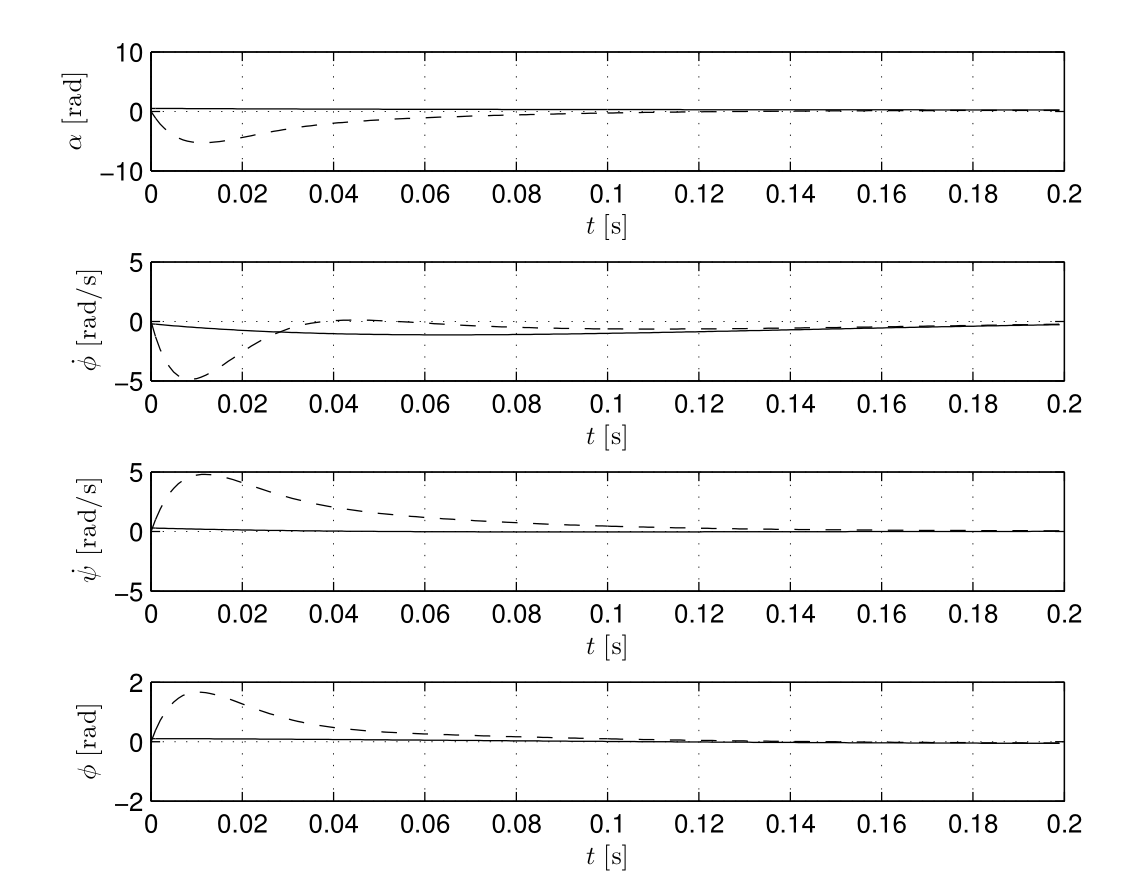
\includegraphics[width=0.9\linewidth]{figures/ObserverIdentityPerformance}
	\caption{Performance of the observer identity. The dashed lines are the state estimates}
	\label{fig:observeridentityperformance}
\end{figure}


\section{REDUCED ORDER OBSERVER}
Another approach is to use an observer of reduced order, due to the degree of redundancy that exists in the observer identity. As two measurements are performed, only two states need to be estimated. For this, a variable transformation is performed through the matrix

\begin{equation}\mathbf{P=
\begin{bmatrix}
V\\
C
\end{bmatrix}}
\end{equation}

Where $\mathbf{V}$ must be chosen in such a way that the matrix $\mathbf{P}$ has the same size as $\mathbf{A}$ and is reversible.

The new transformed vector is:

\begin{equation}\mathbf{\tilde{x}=
	\begin{bmatrix}
	w\\
	y
	\end{bmatrix}}
\end{equation}


The dynamic equation of the observer is given by

\begin{equation}\label{eq:39.reduced.order.observer.dynamic.equation}
\mathbf{
\dot{z} = \left(\bar{A}_{11} - E\bar{A}_{21} \right)z +
\left(\bar{A}_{11}E - E\bar{A}_{21}E +\bar{A}_{12}- E \bar{A}_{22}\right)y + 
\left(\bar{B}_{1}- E\bar{B}_{2}\right)u 
}
\end{equation}


The vector z is obtained by integrating equation (\ref{eq:39.reduced.order.observer.dynamic.equation}) (with zero initial conditions) with only y as input. In this way, the estimate of $\mathbf{w}$ can be calculated as 

\begin{equation}
\mathbf{\hat{w} = z+Ey}
\end{equation}

The estimated transformed variable is given by

\begin{equation}\mathbf{\hat{\tilde{x}}=
	\begin{bmatrix}
	\hat{w}\\
	y
	\end{bmatrix}}
\end{equation}


Finally, the estimation of the states of the system can be obtained by equation

\begin{equation}
\mathbf{
	\hat{x}= P^{-1}\hat{\tilde{x}}
}
\end{equation}

The detailed description of this type of observer can be found in \cite{Luenberger1979introduction}. %Luenberger (1979).

In this technique, the observer dynamics is also adjusted by the matrix $\mathbf{E}$. The eigenvalues of ($\bar{A}_11-E \bar{A} _{21}$) are chosen as
\begin{verbatim}
-96.4481 +61.8839i
-96.4481 -61.8839i
\end{verbatim}

And the matrix $\mathbf{E}$ is obtained by the \emph{place} command of the Matlab program.
The performance of the observer is shown in figure \ref{fig:luenbergerobserverperformance} for the same integration as in figure \ref{fig:stateevolution}. In less than 0.1 seconds the estimated states converge to the values of the states of the linear model representing the system. 

\begin{figure}
	\centering
	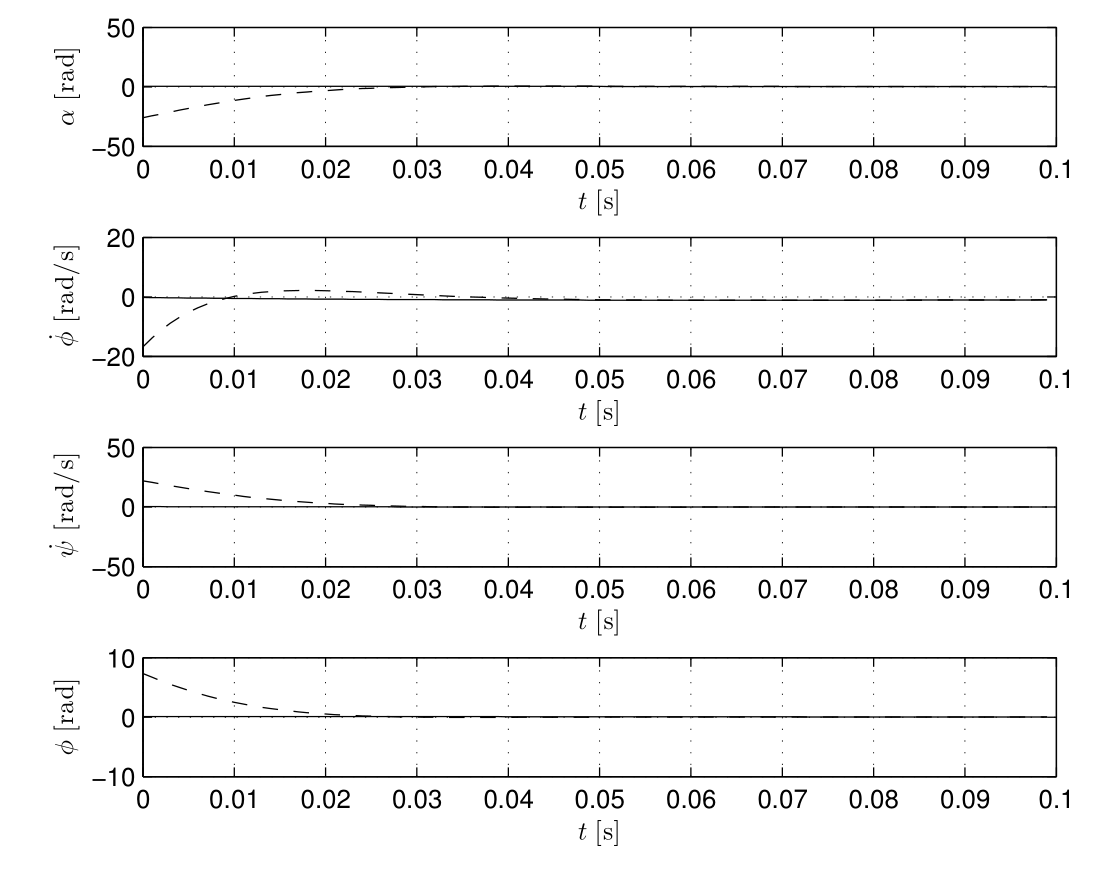
\includegraphics[width=0.9\linewidth]{figures/LuenbergerObserverPerformance}
	\caption{Performance of the Luenberger observer. The dashed lines are the state estimates}
	\label{fig:luenbergerobserverperformance}
\end{figure}



\bibliography{referencias}
\bibliographystyle{apalike}

\end{document}
